%
% File dialogue-2022.tex
%
% Made by Serge Sharoff following the style guide file for COLING-2020,
% see the full story in https://coling2020.org/coling2020.zip

\documentclass[11pt]{article}

\usepackage{dialogue}

\usepackage{ifxetex}
\ifxetex
    \usepackage{fontspec}
    \setromanfont{Times New Roman}
\else
  \usepackage{cmap}
  \usepackage[T2A,T1]{fontenc}
  \usepackage[utf8]{inputenc}
  \usepackage{times}
  \usepackage{latexsym}
  \usepackage{substitutefont}
  \substitutefont{T2A}{\familydefault}{cmr}
\fi

\usepackage[russian,british]{babel}
\usepackage{url}
\usepackage{pgf}

%% MY CODE
\usepackage{float}
\usepackage{array}
\usepackage{amsmath}
%\usepackage{biblatex}
%%

%% For proper formatting of linguistic examples use
%% https://anorien.csc.warwick.ac.uk/mirrors/CTAN/macros/latex/contrib/covington/covington.pdf
\usepackage{covington} %% comment it out if you do not require this option

%% To make citations and references clickable
\usepackage{hyperref}

\renewcommand{\ttdefault}{lmtt}

\dialogfinalcopy % Uncomment this line for the final submission


\title{Interpretable approach to detecting semantic changes based on generated definitions}

\author{ Tatarinov Maksim \\
   HSE University \\
   Nizhny Novgorod, Russia \\
  {\tt tatarinovst0@gmail.com} \\\And
   Demidovsky Aleksandr \\
 HSE University \\
   Nizhny Novgorod, Russia \\
  {\tt monadv@yandex.ru} \\
}

\date{}

\begin{document}
\maketitle
\begin{abstract}
This paper investigates definition modeling as an approach to semantic change detection,
which offers the advantage of providing human-readable explanations, unlike traditional embedding-based approaches that lack interpretability.
Definition modeling leverages large language models to generate dictionary-like definitions based on target words and their contextual usages.
Despite its potential, practical evaluations of this method remain scarce.
In this study, FRED-T5 was fine-tuned using the Small Academic Dictionary for the task of definition modeling.
Both quantitative and qualitative assessments of definition modeling's effectiveness in detecting semantic shifts within the Russian language were conducted.
The approach achieved a Spearman's rank correlation coefficient of 0.815 on the Rushifteval task, demonstrating strong alignment with expert annotations and ranking among the leading solutions.
For interpretability, a visualization algorithm was proposed that displays semantic changes over time.
In the qualitative evaluation, our system successfully replicated manual linguistic analysis of 20 Russian words that had undergone semantic shifts.
Analysis of the generated meanings and their temporal frequencies showed that this approach could be valuable for historical linguists and lexicographers.

  \textbf{Keywords:} Semantic change, definition modeling, definition generation

  \textbf{DOI:} 10.28995/2075-7182-2022-20-XX-XX
\end{abstract}

\selectlanguage{russian}
\begin{center}
  \russiantitle{Интерпретируемый подход к детектированию семантических изменений слов на основе генерируемых определений}

  \medskip \setlength\tabcolsep{2cm}
  \begin{tabular}{cc}
    \textbf{Татаринов Максим} & \textbf{Демидовский Александр}\\
      НИУ ВШЭ & НИУ ВШЭ\\
      Нижний Новгород, Россия & Нижний Новгород, Россия \\
      {\tt tatarinovst0@gmail.com} & {\tt monadv@yandex.ru}
  \end{tabular}
  \medskip
\end{center}

\begin{abstract}
В данной работе исследуется моделирование определений как подход к обнаружению семантических изменений,
который имеет преимущество в виде понятных для человека объяснений,
в отличие от традиционных подходов на основе векторных представлений, страдающих от недостатка интерпретируемости.
Моделирование определений использует большую языковую модель для генерации словарных определений на основе целевых слов и их контекста.
Несмотря на потенциал, практико-ориентированные оценки этого метода остаются ограниченными.
В данном исследовании FRED-T5 была дообучена с помощью Малого академического словаря на задаче моделирования определений.
Были проведены как количественные, так и качественные оценки эффективности моделирования определений в обнаружении семантических сдвигов в рамках русского языка.
Подход достиг коэффициента ранговой корреляции Спирмена 0,815 в задаче Rushifteval, что демонстрирует сильное соответствие экспертным аннотациям, находясь среди лидирующих решений.
Для интерпретируемости был предложен алгоритм визуализации, который отображает семантические изменения во времени.
В качественной оценке наша система успешно воспроизвела ручной лингвистический анализ 20 русских слов, имевших семантическими сдвиги.
Анализ сгенерированных значений и их временных частот показал, что этот подход может быть востребован для исторических лингвистов и лексикографов.

  \textbf{Ключевые слова:} Семантические изменения, моделирование определений, генерация определений

\end{abstract}
\selectlanguage{british}

\section{Introduction}

Static and contextual embeddings excel at capturing semantic relationships for detecting semantic change,
but lack human-readable word descriptions.
Advancements in recent research involve definition generation with language models, which offer more illustrative descriptions~\cite{DefinitionGenerationMainArticle,fedorova-etal-2024-definition}.
It could aid historical linguists and lexicographers in creating dictionaries and language history studies, such as \newcite{TwoCenturies}.
%Moreover, such models could be useful in tasks like sentiment analysis, machine translation, lexical meaning extraction, and semantic disambiguation~\cite{DefinitionModelingReviewAndDatasetAnalysis}.
%For example, lexical sense extraction is used in Sketch Engine where currently the algorithm is unable to provide descriptions of meanings, instead reporting words from the same semantic field.
However, the practical evaluation of this approach remains limited.

The primary objective of this study is to assess the effectiveness of language models in detecting semantic changes in words through the generation of definitions.
%It would include quantitative assessment using an existing shared task for semantic change detection,
%as well as qualitative evaluation by using the approach to reproduce manual linguistic analyses of words known to have undergone semantic shifts.
It would use both quantitative metrics from a shared task and qualitative analysis by reproducing a linguistic analysis of words known to have undergone semantic shifts.

The paper is organized as follows:
Section~\ref{sec:related-work} reviews semantic change detection methods, evaluation methods for classifying errors in generated definitions and a strategy to acquire correct ones for comparison.
Section~\ref{sec:proposed-approach} describes the proposed methodology.
Section~\ref{sec:results-and-discussion} presents the results and discusses their implications.

\section{Related Work}\label{sec:related-work}

\subsection{Approaches to Semantic Change Detection}

Semantic change is understood as change in the polysemy of a word over time.
Although most solutions provide a quantitative measure of semantic change, such as a score or distance between vectors,
to determine the extent of change, recently, a step towards a more explainable approach has been taken~\cite{DefinitionGenerationMainArticle,fedorova-etal-2024-definition}.

There have been multiple approaches to semantic change detection:

\textbf{Static Embeddings.}
Static embeddings provide a fixed representation of a word for the entire corpus.
In the Shiftry~\cite{shiftry}, Word2Vec~\cite{Word2VecOriginal} was utilized to examine semantic shifts by dividing the corpus by years to generate distinct word vectors for each period.

%Although effective until 2020 in tasks like SemEval-2020 Task 1~\cite{semeval2020task},
They need extensive data for stable representations, fail to differentiate multiple meanings of a word,
and independently trained models produce incompatible vector spaces requiring alignment.

\textbf{Contextual Embeddings.}
Contextual models such as BERT~\cite{BERTOriginal} and ELMo~\cite{ELMOOriginal} generate different embeddings for a word depending on its context.
\newcite{GlossReader} fine-tuned the XLM-R model to generate embeddings aligned with dictionary definitions.
\newcite{DeepMistake} trained XLM-R on a large multilingual dataset and RuSemShift data.

The GlossReader approach showed limitations with culturally specific words and depended on predefined senses for visualization,
while the DeepMistake method lacked visualization capabilities.

\textbf{Definition Modeling.}
Definition modeling takes a target word with a usage example to generate a human-readable word definition based on context,
akin to a dictionary entry~\cite{DefinitionGenerationMainArticle},
unlike previous embedding approaches which produce abstract vector representations that are difficult to interpret.

\begin{table}[H]
\centering
\caption{Example of Definition Modeling}
\label{tab:Definition modeling example}
\begin{tabular}{|l|p{10cm}|}
\hline
\textbf{Example Usage} & He started to sleep poorly at night, waking up with a persistent headache. \\
\hline
\textbf{Target Word} & night \\
\hline
\textbf{Generated Definition} & The part of the day from sunset to sunrise. \\
\hline
\end{tabular}
\end{table}

%The interest in definition modeling was initiated by \newcite{noraset2016definition},
%who investigated the use of word vector representations for automatic definition generation, initially focusing on monosemous words.
%Addressing the challenge of polysemy, \newcite{gadetsky-etal-2018-conditional} incorporated usage examples.
%Challenges in the task include dealing with out-of-vocabulary words and ensuring the definitions are specific and accurate~\cite{huang-etal-2021-definition}.
%Advanced models like Flan-T5 have enhanced definition generation by demonstrating high data correlation and outperforming traditional embeddings in clustering~\cite{DefinitionGenerationMainArticle}.
\newcite{DefinitionGenerationMainArticle} proposed using generated definitions as semantic embeddings for words, enabling semantic change detection.
\newcite{fedorova-etal-2024-definition} researched definition modeling for the task of semantic change detection finding it successful.

The main limitation of the approaches employing embeddings is their non-interpretability.
The best case is the DeepMistake, whose visualization is limited to predetermined senses.

As for definition modeling, qualitative evaluation in \newcite{fedorova-etal-2024-definition} is limited, as they leave \("\)in-practice\("\) evaluation for future research.
Also, they used an unsupervised approach for an evaluation, while the proposed approach involved fine-tuning the vectorizer.

\subsection{Classification of Errors in Generated Definitions}

Studies by \newcite{huang-etal-2021-definition} and \newcite{noraset2016definition} have proposed classifications for errors in generated definitions.
Their work identified the following types:

\begin{table}[H]
    \centering
    \caption{Types of Errors in Generated Definitions}
    \begin{tabular}{|p{3.5cm}|p{6.5cm}|p{5.5cm}|}
        \hline
        \textbf{Type} & \textbf{Russian Example} & \textbf{English Example (Translation)} \\ \hline
        \textbf{Over-specification} & кофе -- горячий, горький напиток из жареных бразильских зерен & coffee -- a hot, bitter beverage made from roasted Brazilian beans \\ \hline
        \textbf{Under-specification} & капитан -- член команды. & captain -- team member \\ \hline
        \textbf{Self-referential} & самосознание -- состояние, при котором у человека присутствует самосознание & self-awareness -- a state in which a person has self-awareness \\ \hline
        \textbf{Wrong Part of Speech} & стекло -- переместиться вниз, сбежать (о жидкости) & glass/spilt -- to move down, escape (of a liquid) \\ \hline
        \textbf{Opposite Meaning} & внутрь -- ненаправленный в центр & inward -- non-directed to the center \\ \hline
        \textbf{Close Semantics} & машина -- устройство с автоматическими функциями & machine -- a device with automatic functions \\ \hline
        \textbf{Redundancy or Excessive Use of Generic Phrases} & спутник -- тот, кто совершает путь, путь вместе с кем-л. & companion -- one who makes a journey, journey together with someone \\ \hline
        \textbf{Incorrectness} & первый -- следующий после всех остальных в списке предметов & first -- next after all other items in the list \\ \hline
        \textbf{Correct} & винодельня -- заведение, помещение для изготовления вина & vineyard -- establishment, premises for wine production \\ \hline
    \end{tabular}
    \label{tab:error_classification}
\end{table}

\subsection{Acquiring correct definitions}

\newcite{SemanticDefinitionsAndAnalysis} outlines a method of generalizing dictionary definitions for determining correct semantic description of words,
emphasizing the integration of diverse dictionary definitions to capture the full meaning.
This procedure involves compiling all available definitions, differentiating meanings based on denotative principles, and synthesizing a unified semantic structure,
with the final step organizing meanings from core to peripheral, accompanied by usage examples.

\section{Proposed Approach}\label{sec:proposed-approach}

\subsection{Fine-tuning LLM}

A generative large language model \( M \) is trained on a dataset \( D = \{(w_i, c_i, d_i)\}_{i=1}^{N} \),
where each tuple contains a word \( w \), its context \( c \), and a corresponding definition \( d \).
The model learns to generate an accurate definition \( \hat{d} = M(w, c) \) by minimizing the cross-entropy loss between its predicted token probabilities and the reference definitions:

\begin{equation}
L(M) = \sum_{i=1}^{N} \text{loss}(M(w_i, s_i), d_i),
\end{equation}

\subsection{Testing}

\textbf{Intrinsic evaluation} is conducted using a test subset \( D_{\text{test}} \) of the dataset \( D \)
to assess the quality of generated definitions \( \hat{d}_j = M(w_j, c_j) \)
compared to reference definitions \( d_j \) using string similarity metrics, defined as:

\begin{equation}
\text{metric} = \frac{1}{M} \sum_{j=1}^{P} \text{similarity}(\hat{d}_j, d_j)
\end{equation}

where \( \text{similarity} \) measures the match between definitions, ranging from 0 (no similarity) to 1 (identical).

\textbf{Extrinsic evaluation} assesses the model's performance on
a semantic change detection task with test set \( S = \{(w_k, g_{k,(t_i,t_j)})\}_{k=1}^{Q} \),
where \( w_k \) represents a target word, \( g_{k,(t_i,t_j)} \) its gold semantic change score for the transition between periods \( t_i \) and \( t_j \), and \( Q \) is the number of words in the test set.

For each word \( w_k \) in the test set,
a set of usage contexts \( U_{k,t} = \{u_{k,t,1}, u_{k,t,2}, \dots, u_{k,t,n}\} \) is sampled from each time period \( t \in \{t_1, t_2, t_3\} \) of the diachronic Russian National Corpus~\cite{Ruscorpora},
where \( n \) is 100 or all if fewer available, in a similar way to \newcite{DeepMistake}.
For each period transition, the usages are paired, and definitions \( \hat{d}_{k1}, \hat{d}_{k2}\) are generated by the model for each pair.

These definitions are then vectorized \( \vec{d}_{k1}, \vec{d}_{k2} \) using a vectorizer \( V \).
The distance between the vectorized definitions \( dist(\vec{d}_{k1}, \vec{d}_{k2}) \) is calculated and converted to scores ranging from 1 (senses unrelated) to 4 (identical).

The mean values of the ratings for each word are compared with the gold scores from the task
using Spearman's rank correlation.

\subsection{Visualization}

To illustrate semantic changes over time, generated definitions are transformed into vector representations using a vectorizer \( V \).

A clustering algorithm \( C \) is then applied to group similar definitions.

For each cluster \( K_j \), a prototypical definition \( \hat{d}_{\text{proto}} \) is selected,
which is defined as original definition whose vector \( \vec{d}_{\text{proto}} \) is the closest to the center of the cluster (centroid).

Let \( \vec{c_j} \) be the centroid of cluster \( K_j \):

\begin{equation}
\vec{d}_{\text{proto}, j} = \arg\min_{\vec{d} \in K_j} dist(\vec{d}, \vec{c_j})
\end{equation}

where \( dist \) is a distance metric.

Bar charts are then created to display the frequency of different meanings over time.

\subsection{Qualitative Analysis}

A qualitative assessment begins with the selection of words known to have undergone semantic shifts based on existing linguistic research.
Usage examples for these words are obtained from different time periods using a diachronic corpus.
The trained model is applied to generate definitions for each word usage.
The obtained definitions are compared with information from semantic descriptions of words,
written based on \newcite{SemanticDefinitionsAndAnalysis} method of generalizing dictionary definitions,
and classified according to the error types in Table~\ref{tab:error_classification}.
Finally, changes in the frequency of meanings over time provided by the visualizations are examined and compared with historical usage data.

\section{Results and Discussion}\label{sec:results-and-discussion}

\subsection{Model}

FRED-T5-1.7B was chosen due to its performance in processing the Russian language~\cite{FRED-T5}.
At the time of selection, it was the top performer on the RussianSuperGLUE benchmark~\cite{RussianSuperGLUE}, with a score of 0.762.

\subsection{Training Data}\label{subsec:training-data}

FRED-T5-1.7B was trained on a dataset derived from \("\)Small academic dictionary\("\) (MAS)~\cite{MAS1981}.
%Data extraction was performed using a Python-based scraper.

The dataset was cleaned to remove usage labels, entries without usage examples or without informative definitions, such as \textit{Состояние по знач. глаг. линять} [\textit{State by the meaning of the verb "to shed"}],
and those that provided grammatical rather than lexical information, such as \textit{наречие к причастию приглашающий} [\textit{Adverb to the participle "inviting"}].
The resulting dataset of 122,350 entries was partitioned into training, validation, and test sets with a 90\%/5\%/5\% split.

Each entry was formatted and began with the word \("\)Контекст\("\) [\("\)Context\("\)] followed by a usage example, then the phrase \("\)Определение слова\("\) [\("\)Word definition\("\)], and the word itself.\footnote{A special denoiser token \texttt{<LM>}, dedicated to the task of text continuation, was utilized.}

\subsection{Evaluation Data}

The \textit{RuShiftEval} competition's test set~\cite{rushifteval} was utilized for evaluation.
The task focuses on detecting semantic changes in Russian nouns across three historical transitions:
RuShiftEval-1 (Pre-Soviet:Soviet), RuShiftEval-2 (Soviet:Post-Soviet), and RuShiftEval-3 (Pre-Soviet:Post-Soviet).
The competition provided a test set of gold change scores for 99 Russian nouns corresponding to the transitions.
%Evaluation was conducted using Spearman's rank correlation to measure the alignment between the approach's results and the gold scores.

\subsection{String Similarity Metrics in Model Testing}

BLEU~\cite{BLEUScore}, ROUGE-L~\cite{ROUGE}, and BERT-F1~\cite{BERTScore} metrics from the \textit{evaluate} library~\cite{Evaluate} were employed for the definitions generated using the test part of the MAS dataset.
BLEU measures n-gram overlap between texts, ROUGE-L focuses on the longest common subsequence,
and BERT-F1 leverages contextual embeddings for semantic similarity.
The evaluation results\footnote{Out of 100, higher is better.} are presented in Table~\ref{tab:Similarity_metrics}.

\begin{table}[H]
\centering
\caption{Fine-tuning Results of FRED-T5-1.7B on the MAS Dataset}
\label{tab:Similarity_metrics}
\begin{tabular}{|l|c|}
\hline
\textbf{Metric}                  & \textbf{Value} \\
\hline
BLEU            & 11.02                  \\
\hline
ROUGE-L           & 29.36                  \\
\hline
BERT-F1          & 75.22                  \\
\hline
\end{tabular}
\end{table}

%\begin{table}[H]
%\centering
%\caption{Fine-tuning Results of FRED-T5-1.7B on the MAS Dataset}
%\label{tab:Similarity_metrics}
%\begin{tabular}{|c|c|c|c|}
%\hline
%\textbf{Metric}   & BLEU  & ROUGE-L & BERT-F1 \\ \hline
%\textbf{Value}    & 11.02 & 29.36   & 75.22    \\ \hline
%\end{tabular}
%\end{table}

Low BLEU and ROUGE-L scores indicate that the model generates definitions differently from the test set,
although high BERT-F1 scores imply semantic similarity.

%For example, both the expected definition “ставший тощим, отощавший [becoming thin, emaciated]”
%and the model-generated “сильно исхудавший от недоедания [severely emaciated from malnutrition]” are correct
%but share no common tokens, resulting in BLEU and ROUGE-L scores of 0, with BERT-F1 scoring 70.39.

At this stage, self-referential errors were fixed by excluding tokens related to the target word from being sampled in the model's output.
%For example, for the context \textit{...ничего не мог сделать, чтобы восстановить в семье прежний порядок. [...couldn't do anything to restore the previous order in the family.]},
%and the target word \textit{восстановить [restore]}, the initial output was ‘привести в прежнее состояние; восстановить’.
%After excluding tokens related to the target word, the model generated ‘привести в прежнее состояние, положение’.

\subsection{Rushifteval Testing}

%Our approach to solving the task is similar to \newcite{DeepMistake} and involves reproducing the RuShiftEval annotation effort.
%For 99 test words from the Rushifteval competition, 100 sentences (or all, if there were fewer) were randomly sampled for each period from the diachronic sub-corpus of the Russian National Corpus~\cite{Ruscorpora}.
%For each period transition, the usages were paired, and the model generated definitions for each pair.
The paraphrase-multilingual-mpnet-base-v2 model~\cite{Vectorizer}, additionally fine-tuned on RuSemShift, a similar dataset~\cite{rusemshift}, was used to vectorize definitions.
The distances between the definitions were calculated using the cosine distance.
%After that, mean values of the ratings for each word were compared with the gold scores using Spearman's rank correlation.
Results were compared against approaches from the Rushifteval task,
as shown in Table~\ref{tab:Rushifteval_all}.

\begin{table}[H]
\centering
\caption{Algorithm Results Compared to Rushifteval Teams}
\label{tab:Rushifteval_all}
\begin{tabular}{|m{3.5cm}|m{2cm}|m{4cm}|m{3cm}|}
\hline
\textbf{Team} & \textbf{Average} & \textbf{Word Representation Type} & \textbf{Model Used} \\
\hline
\textbf{DeepMistake (post-competition)} & \textbf{0.850} & \textbf{Contextual Emb.} & \textbf{XLM-R} \\
\hline
\textbf{Proposed Approach} & \textbf{0.815} & \textbf{Generated Definitions} & \textbf{FRED-T5-1.7B} \\
\hline
GlossReader & 0.802 & Contextual Emb. & XLM-R \\
\hline
DeepMistake & 0.791 & Contextual Emb. & XLM-R \\
\hline
vanyatko & 0.720 & Contextual Emb. & RuBERT \\
\hline
Other 10 Teams & 0.457-0.178 & \ldots & \ldots \\
\hline
\end{tabular}
\end{table}

The proposed approach outperforms most entries in the Rushifteval competition.

\begin{table}[H]
\centering
\caption{Comparison with definition generation approaches}
\label{tab:Definition_modeling_results}
\begin{tabular}{|m{4cm}|m{2.5cm}|m{2.5cm}|m{2.5cm}|m{2.5cm}|}
\hline
\textbf{Method} & \textbf{RuShiftEval-1} & \textbf{RuShiftEval-2} & \textbf{RuShiftEval-3} & \textbf{Base Model} \\
\hline
\textbf{Proposed Approach without vectorizer fine-tuning} & \textbf{0.722} & \textbf{0.763} & \textbf{0.749} & \textbf{FRED-T5-1.7B} \\
\hline
\newcite{fedorova-etal-2024-definition} & 0.488 & 0.462 & 0.504 & MT0-XL \\
\hline
\end{tabular}
\end{table}

A shown in Table~\ref{tab:Definition_modeling_results},
the proposed approach significantly outperforms the results of \newcite{fedorova-etal-2024-definition}.
The vectorizer fine-tuning step was omitted to ensure that the results are directly comparable.

It could be noted that \newcite{fedorova-etal-2024-definition} appears to retain unhelpful definitions in the training data,
unlike proposed approach in~\ref{subsec:training-data}, possibly resulting in their model reproducing non-informative patterns and the lower performance of their approach.

%It could be noted that \newcite{fedorova-etal-2024-definition} does not seem to clean the training dataset in the way done in~\ref{subsec:training-data},
%possibly contributing to the lower performance of their approach.

\subsection{Visualization}

Generated word vectors were clustered using the DBSCAN algorithm.
Each cluster is represented by a prototypical definition closest to its centroid.
DBSCAN parameters (\texttt{eps} and \texttt{min\_samples}) are manually tuned by incremental adjustment to ensure the formation of cohesive clusters.
%as there is no predefined optimal method for clustering semantically similar definitions.
Then, the temporal distribution of these meanings is displayed using bar charts, as shown in Figure~\ref{fig:Машина_example}.

\begin{figure}[H]
    \centering
    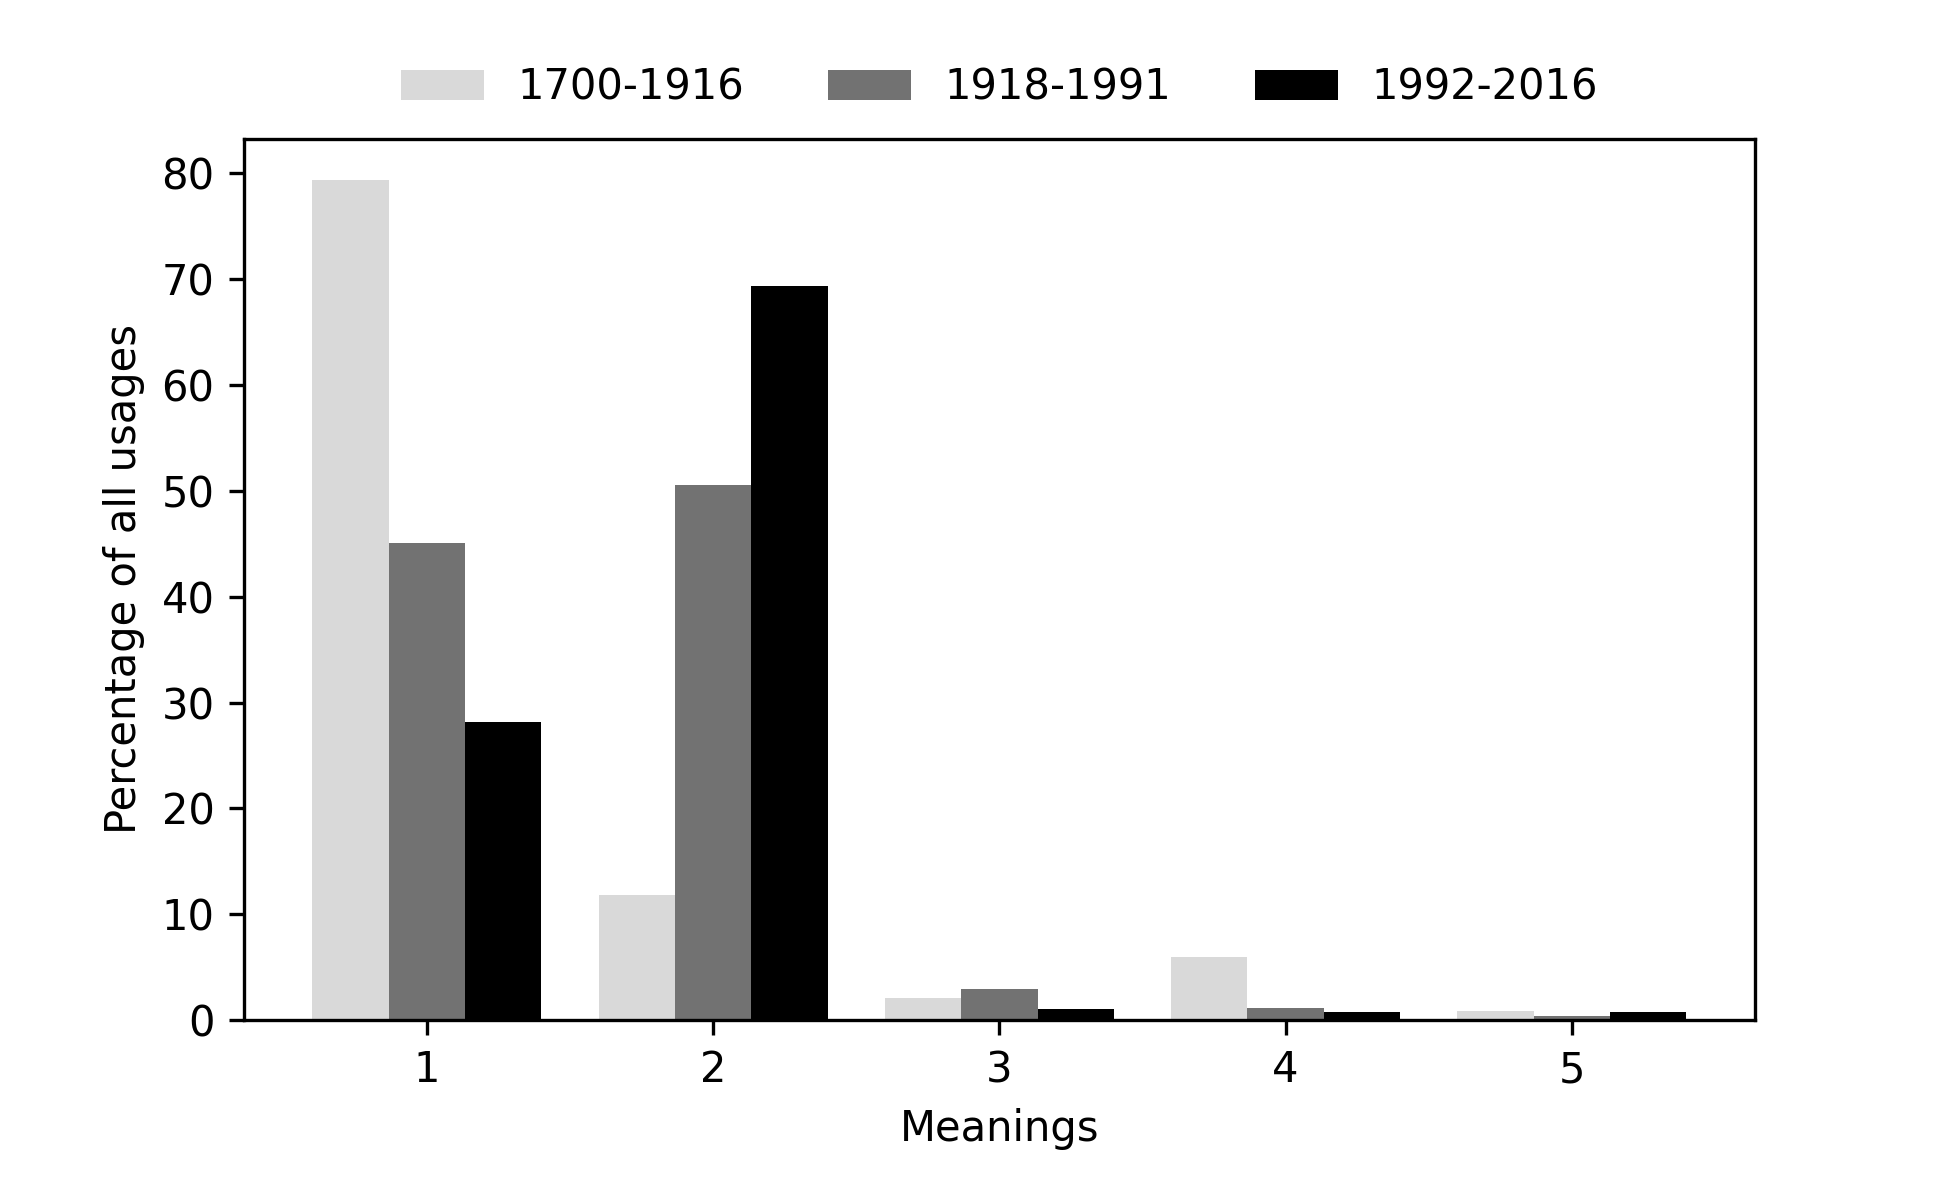
\includegraphics[width=0.8\textwidth]{img/mashina_minimal}
    \caption{Semantic Shift of the Word \textit{машина [machine/car]} (Parameters: eps=0.14, min\_samples=5)}
    \label{fig:Машина_example}
\end{figure}

\begin{center}
    \begin{minipage}{0.7\textwidth}
        \centering
        \textbf{Meanings for \textit{машина [machine/car]}:}
        \begin{enumerate}
            \item A device or instrument for a specific task.
            \item An automobile or vehicle.
            \item An aircraft or helicopter.
            \item A mechanically or thoughtlessly acting person.
            \item A system of institutions or organizations.
    \end{enumerate}
    \end{minipage}
\end{center}

\subsection{Qualitative Analysis}

For deeper examination, 20 words exhibiting semantic shifts from \textit{Two Centuries in Twenty Words}~\cite{TwoCenturies} were selected:
\textit{знатный [noble]}, \textit{кануть [to disappear]}, \textit{классный [classy/cool]}, \textit{мама [mom]}, \textit{машина [machine/car]},
\textit{молодец [young man/attaboy]}, \textit{пакет [bag/package]}, \textit{передовой [advanced]}, \textit{пионер [pioneer]},
\textit{пожалуй [perhaps]}, \textit{пока [until/bye]}, \textit{привет [hello]}, \textit{пружина [spring]}, \textit{публика [public]},
\textit{свалка [landfill/fight]}, \textit{сволочь [bastard]}, \textit{стиль [style]},
\textit{тётка [aunt]}, \textit{тройка [three/a set of three]}, \textit{червяк [worm]}.
The usages were extracted from the diachronic sub-corpus of Russian National Corpus~\cite{Ruscorpora}.

For each word, 300 instances were randomly sampled for each period of the corpus (pre-Soviet, Soviet, post-Soviet).
The model generated definitions for each occurrence, followed by the creation of corresponding visualizations.

Next, the semantics of each word based on multiple dictionaries were described following \newcite{SemanticDefinitionsAndAnalysis}.
To ensure comprehensive meaning descriptions, we synthesized information from 3 modern Russian dictionaries:
\textit{Big Explanatory Dictionary}~\cite{TolkovyKuznetsov}, \textit{Dmitriev's Explanatory Dictionary of the Russian Language}~\cite{TolkovyDmitriev}, and \textit{Ozhegov and Shvedova's Explanatory Dictionary}, in addition to \textit{Two Centuries in Twenty Words}.
Usage labels were omitted since the model wasn't trained to generate them.

The manually obtained semantic descriptions were compared with those in the visualization,
and changes in their usage across periods for meanings corresponding to those in \textit{Two Centuries in Twenty Words} were analyzed.

\subsection{Qualitative Analysis of Generated Definitions}

As a result of generalizing dictionary definitions, 121 meanings were compiled for 20 words.
A total of 83 definitions were obtained using the proposed approach.
Thus, excluding 5 incorrect definitions, 64.4\% of the meanings were identified.

\begin{table}[H]
\centering
\caption{Types of Definitions and Their Counts}
\label{tab:definitions_classification}
\begin{tabular}{|>{\raggedright\arraybackslash}p{8cm}|c|c|}
\hline
\textbf{Type of Definition} & \textbf{Count} & \textbf{Percentage} \\ \hline
Correct & 57 & 68.67\% \\ \hline
Close & 10 & 12.04\% \\ \hline
Incorrect & 5 & 6.02\% \\ \hline
Insufficiently Specific & 3 & 3.61\% \\ \hline
Redundancy or Excessive Use of General Phrases & 4 & 4.81\% \\ \hline
Close, Redundancy or Excessive Use of General Phrases & 1 & 1.20\% \\ \hline
Overly Specific & 3 & 3.61\% \\ \hline
Self-reference & 0 & 0.00\% \\ \hline
Opposite Meaning & 0 & 0.00\% \\ \hline
Incorrect Part of Speech & 0 & 0.00\% \\ \hline
\end{tabular}
\end{table}

As shown in Table~\ref{tab:definitions_classification}, the majority of definitions are correct without any errors or shortcomings (68.67\%).

Common issues include close or incorrect meanings, such as defining \textit{червяк [worm]} as an adult insect or describing \textit{пожалуй [perhaps]} as a conjunction.
Redundancy is present, exemplified by the repetitive “chaotic” in the definition of \textit{свалка [landfill/fight]} (‘Беспорядочная, беспорядочная схватка’),
possibly due to the abundance of synonymous expressions in the training dataset, a common method in lexicology.
Additionally, some definitions lack specificity, such as describing \textit{мама [mom]} simply as ‘a tender address to a woman.’
These problems may arise from the model's limited world knowledge.

Another issue is insufficient context, leading to ambiguity in distinguishing meanings,
as seen with \textit{пионер [pioneer]} in \textit{Pioneers listen to this and admire it [Пионеры слушают это и восхищаются].}

\subsection{Statistical Analysis of Semantic Shifts}

For most of the words, the visualizations partially or fully align with the data from \textit{Two Centuries in Twenty Words},
except for the word \textit{пока [until/bye]}, where the visualization results contradict the study’s findings.
Overall, main meaning changes consistent with the book's data were identified in 12 out of 20 words.
Additionally, changes partially aligned in 4 other words.

One of the best visualizations was created for the word \textit{пакет [bag/package]}.
7 definitions were identified correctly, 4 of which appear only in the post-Soviet period.

\begin{figure}[H]
    \centering
    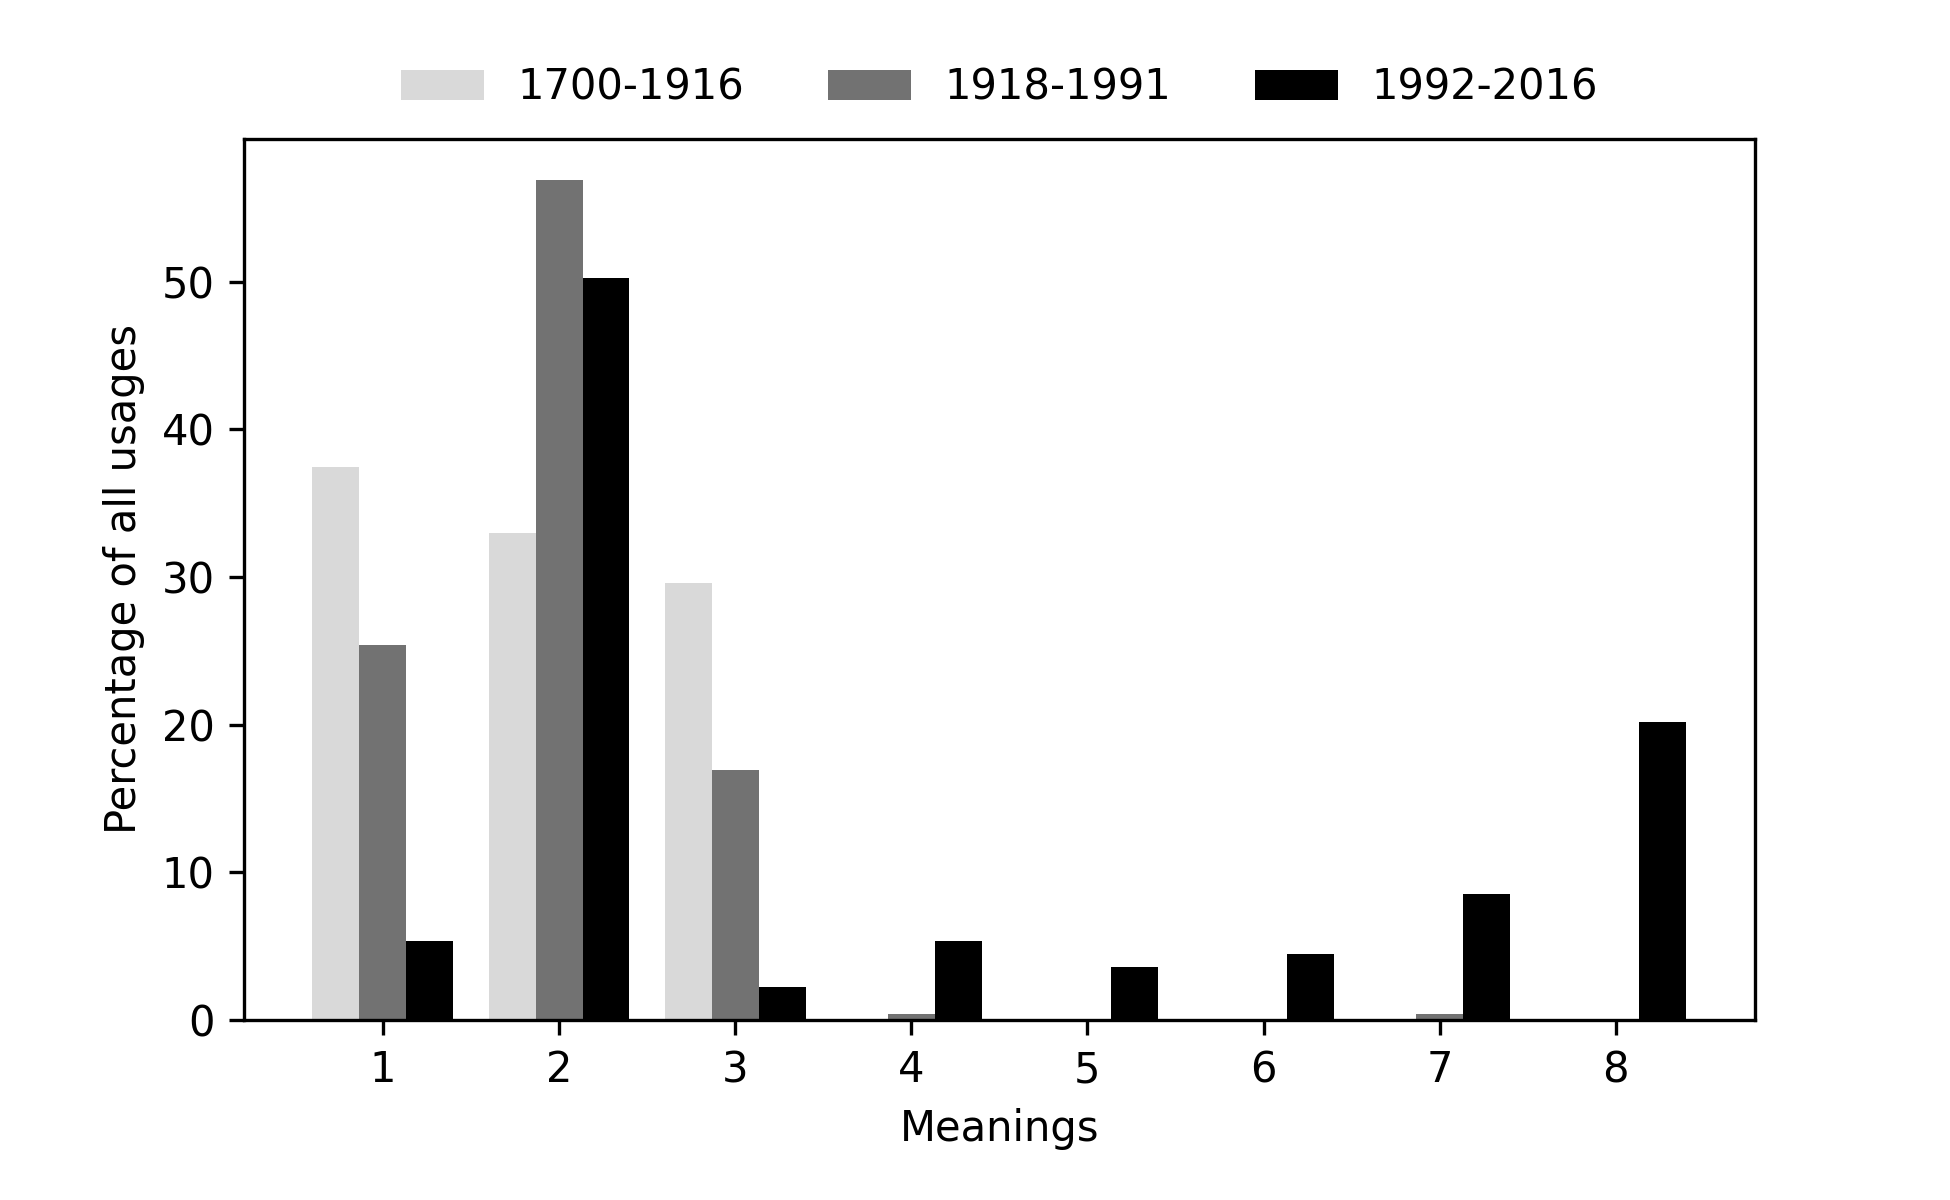
\includegraphics[width=0.8\textwidth]{img/paket_minimal}
    \caption{Semantic Shift of the Word \textit{пакет [bag/package]} (Parameters: eps=0.11, min\_samples=8)}
    \label{fig:paket_example}
\end{figure}

\begin{center}
    \begin{minipage}{0.7\textwidth}
        \centering
        \textbf{Meanings for \textit{пакет [bag/package]}:}
        \begin{enumerate}
            \item A letter, parcel, etc., in such a form.
            \item A paper or fabric pouch for storing, transporting, etc.
            \item A letter, parcel, etc., sealed in such an envelope.
            \item A collection of homogeneous, related objects, phenomena, etc.
            \item A collection of software tools united by a certain criterion.
            \item A part of something belonging to someone under certain conditions. (marked as incorrect)
            \item A collection of homogeneous objects, documents, etc.
            \item A collection of shares of a joint-stock company.
        \end{enumerate}
    \end{minipage}
\end{center}

A comprehensive analysis is not feasible for \textit{публика [public]} and \textit{кануть [to disappear]},
because \textit{Two Centuries in Twenty Words} does not provide sufficient usage frequency diagrams for their meanings.

Similarly, for \textit{сволочь [bastard]}, only 2 out of 4 meanings were detected by the proposed approach (\textit{употребляется как бранное слово [used as a swear word]} and \textit{о подлом, гнусном человеке [referring to a vile, despicable person]}),
both falling under ‘Индивидуальное оскорбление [Individual insult]’ in the book.

\section*{Conclusion}

The study demonstrated the effectiveness of definition modeling in detecting and visualizing semantic shifts in the Russian language.
A FRED-T5-1.7B model, fine-tuned on the MAS dictionary, was used to generate context-based word definitions.
The model demonstrated high BERTScore similarity metrics on the test set,
performed among the top solutions on the Rushifteval shared task and outperformed the results of \newcite{fedorova-etal-2024-definition}.
A visualization algorithm was developed to represent semantic changes over time,
allowing for reproducing a manual effort of studying semantic changes for a set of 20 words.
Qualitative analysis of the results revealed that 68.67\% of generated definitions were fully correct,
with main meaning changes accurately detected in 12 out of 17 words available for analysis and partial alignment in 4 others.
This shows that the approach could aid historical linguists and lexicographers in linguistic studies.

%This visualization approach offers the advantage of identifying arbitrary meanings without requiring predefinition by the researcher, unlike methods such as \newcite{GlossReader},
%which can be beneficial for exploring new meanings or those not captured in standard dictionaries.

The findings can be applied to assess the extent of semantic shifts in lexemes, providing visualizations and definitions for each identified meaning.
%Furthermore, the model can enhance natural language processing tasks such as sentiment analysis, machine translation, and disambiguation of semantic ambiguity~\cite{DefinitionModelingReviewAndDatasetAnalysis}.

Future research directions might include incorporating multiple dictionaries as training data or utilizing more advanced LLMs.

The code for this project and the model are available on GitHub: \url{https://github.com/tatarinovst2/work-definition-modeling}


%\section*{Acknowledgements}
%
%The acknowledgements should go immediately before the references.  Do
%not number the acknowledgements section. Do not include this section
%when submitting your paper for review.

% include your own bib file like this:
\bibliography{dialogue}
\bibliographystyle{dialogue}

%\begin{thebibliography}{}
%
%\end{thebibliography}

\end{document}
